%% distro.tex
%% Copyright 2015 Gaël PORTAY <gael.portay@gmail.com>
%
% This work may be distributed and/or modified under the
% conditions of the LaTeX Project Public License, either version 1.3
% of this license or (at your option) any later version.
% The latest version of this license is in
%   http://www.latex-project.org/lppl.txt
% and version 1.3 or later is part of all distributions of LaTeX
% version 2005/12/01 or later.
%
% This work has the LPPL maintenance status `maintained'.
%
% The Current Maintainer of this work is Gaël PORTAY.
%
% This work consists of the file distro.tex.

\documentclass[a4paper]{article}
\usepackage{caption}
\usepackage{graphicx}
\usepackage{hyperref}
\usepackage{listings}
\usepackage[T1]{fontenc}
\usepackage[utf8]{inputenc}
\usepackage[francais]{babel}

\lstloadlanguages{[ANSI]C,sh,make}

\title{Ma première distribution Linux faite maison}
\author{Gaël PORTAY}
\date{\today}

\begin{document}
\sloppy
\maketitle

\tableofcontents

\clearpage
\part{Le noyau}

\section{Première compilation}

Entrons directement dans le vif du sujet et attaquons par la compilation d'un noyau \textit{Linux} ! Nous allons compiler un noyau pour l'architecture hôte : la machine sur laquelle vous travaillez actuellement\footnote{Dans un premier temps, je supposerai que vous travailler sur une machine à base de processeur \textit{Intel x86}. Les extraits de code disponibles à travers ce document sont donnés pour cette architecture. Si vous travaillez sur une autre architecture (exemple : \textit{PowerPC} (\textit{PPC})), vous devrez adapter ces extraits pour votre machine. J'adapterai ces extraits plus tard pour qu'ils soient génériques et puissent être utilisés sur n'importe quelle architecture.}.\\

Je n'aborderai pas ici les concepts de la \textit{compilation croisée}. «~La compilation quoi ?!? croisée ?!?~». Hum... le plus simple est de consulter la page \textit{Wikipédia} sur la \textit{compilation croisée}\footnote{\url{https://fr.wikipedia.org/wiki/Compilateur\#Compilation\_crois.C3.A9e}}. Grosso modo, on compile un programme destiné à être exécuté sur une architecture cible autre que l'architecture hôte, celle sur laquelle on est entrain de compiler. Vous n'y êtes toujours pas ?!? Plus simplement, on compile quelque chose sur notre \textit{PC} à base de processeur \textit{Intel} (\textit{x86}) destiné à être utiliser sur un \textit{Raspberry-PI} (\textit{ARM}). C'est bon vous y êtes ?!? Avec un exemple c'est toujours plus facile à comprendre...\\

Vous êtes prêts ?!? Alors c'est parti !\\

\subsection{Les fichiers sources}

Nous allons avoir besoin des fichiers sources de \textit{Linux}. Pour cela, rien de plus simple : allons sur le site \href{http://www.kernel.org}{kernel.org} pour télécharger la dernière version stable\footnote{A l'heure où j'écris ces lignes, la dernière version stable est la version 4.3.}.\\

La règle \textit{Makefile}, ci-dessous, automatise le téléchargement et le désarchivage de la dernière version stable. Vous pouvez la réutiliser en effectuant un copier/coller dans un fichier \textit{Makefile} et ensuite exécuter la commande suivante : \lstset{language=sh}\lstinline{make linux_download}.\\

\lstset{language=make}
\lstinputlisting[firstline=32,lastline=35,breaklines]{../kernel/Makefile}

Pour le reste de ce document, nous supperons que les fichiers sources sont dans le répertoire \textbf{./linux}.\\

\subsection{make}

Nous y voilà, nous sommes fin prêt pour compiler notre premier noyau ! Excitez, non ?!? Allez, on est parti. Ouvrez un terminal (si ce n'est pas déjà fait) et lancez la commande : \lstset{language=sh}\lstinline{cd linux && make} et...

\begin{verbatim}
$ make
  HOSTCC  scripts/basic/fixdep
  HOSTCC  scripts/kconfig/conf.o
  SHIPPED scripts/kconfig/zconf.tab.c
  SHIPPED scripts/kconfig/zconf.lex.c
  SHIPPED scripts/kconfig/zconf.hash.c
  HOSTCC  scripts/kconfig/zconf.tab.o
  HOSTLD  scripts/kconfig/conf
scripts/kconfig/conf  --silentoldconfig Kconfig
***
*** Configuration file ".config" not found!
***
*** Please run some configurator (e.g. "make oldconfig" or
*** "make menuconfig" or "make xconfig").
***
scripts/kconfig/Makefile:37: recipe for target 'silentoldconfig' failed
make[2]: *** [silentoldconfig] Error 1
Makefile:531: recipe for target 'silentoldconfig' failed
make[1]: *** [silentoldconfig] Error 2
  SYSTBL  arch/x86/entry/syscalls/../../include/generated/asm/syscalls_32.h
  SYSHDR  arch/x86/entry/syscalls/../../include/generated/uapi/asm/unistd_32.h
  SYSHDR  arch/x86/entry/syscalls/../../include/generated/uapi/asm/unistd_64.h
  SYSHDR  arch/x86/entry/syscalls/../../include/generated/uapi/asm/unistd_x32.h
  HOSTCC  arch/x86/tools/relocs_32.o
  HOSTCC  arch/x86/tools/relocs_64.o
  HOSTCC  arch/x86/tools/relocs_common.o
  HOSTLD  arch/x86/tools/relocs
make: *** No rule to make target 'include/config/auto.conf', needed by 'include/config/kernel.release'.  Stop.
\end{verbatim}

C'était trop beau pour être vrai... compiler son noyau n'est pas aussi simple ! \textit{Linux} est une noyau \textit{monolithique} \textit{modulaire} qui supporte plusieurs \textit{architectures} (promis, je ne voulais pas offenser). Comprenez simplement que le projet a besoin d'être configuré avant de pouvoir être compilé avec un vulgaire \lstset{language=sh}\lstinline{make}.\\

\clearpage
\section{Configuration}

\textit{Linux} utilise le langage \textit{\href{https://www.kernel.org/doc/Documentation/kbuild/kconfig-language.txt}{Kconfig}} pour décrire ses options de configurations. Ces options sont définis dans les fichiers \textbf{Kconfig}. Ils sont présent un peu partout dans les répertoires des fichiers sources, à l'image des \textit{Makefiles}.\\

Il existe plusieurs \textit{front-ends} (interfaces) pour afficher le menu de configuration du noyau. Généralement, les développeurs (ou «~Kernel Hackers~») utilisent la bonne vielle interface en \textit{ncurses}, invoquée via le \textit{Makefile} et sa règle \textbf{menuconfig} (\lstset{language=sh}\lstinline{make menuconfig}). Il existe également d'autres interfaces comme \textbf{config} (en ligne de commande), \textbf{nconfig} (nouvelle interface \textit{ncurses}), \textbf{xconfig} (interface \textit{Qt}) et \textbf{gconfig} (interface \textit{GTK+}).\\

Revenons à nos moutons... Lorsque notre première commande \lstset{language=sh}\lstinline{make} a échouée, vous avez surement remarqué le message suivant :
\begin{verbatim}
***
*** Configuration file ".config" not found!
***
*** Please run some configurator (e.g. "make oldconfig" or
*** "make menuconfig" or "make xconfig").
***
\end{verbatim}

Le fichier \textbf{.config} est manquant ! Ce fichier contient la configuration du noyau. C'est une simple liste des options qui seront compilés ou non, intégré à l'image du noyau ou disponible via un module.\\

Bien entendu, les sources du noyau viennent sans aucune configuration. Nous allons donc devoir générer cette configuration.\\

\subsection{menuconfig}

Allez, on se fait une petite frayeur : configurons notre noyau en exécutant la commande \lstinline{make menuconfig}\footnote{Nous allons avoir besoin du paquet de développement de \textit{ncurses}. Si vous n'y arrivez pas, passez simplement cette partie, elle n'est pas essentielle}.\\

\begin{figure}
\label{fig:make_menuconfig}
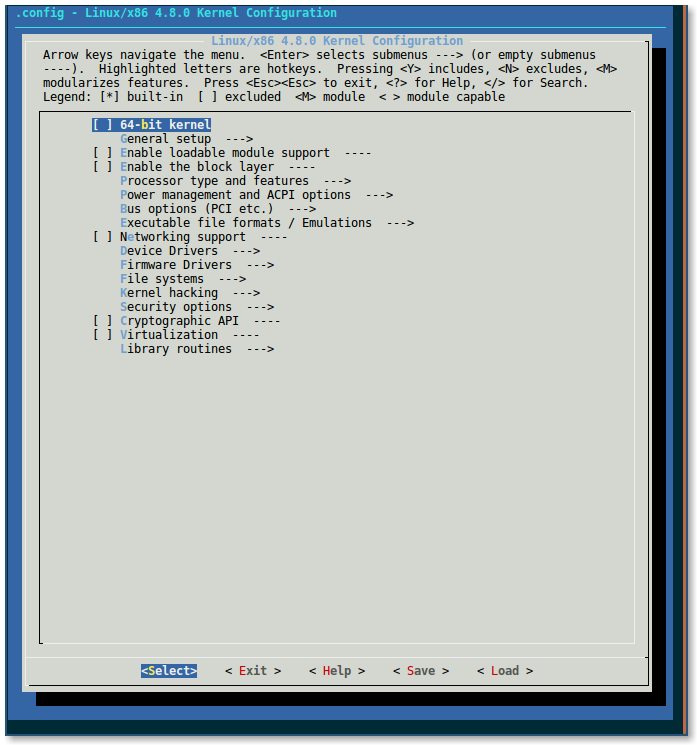
\includegraphics[scale=0.5]{../res/make-menuconfig.png}
\caption{make menuconfig}
\end{figure}

La figure~\ref{fig:make_menuconfig} montre le menu principal de configuration du noyau. Vous pouvez vous balader dans les sous-menus avec les flèches \textit{haut} et \textit{bas} ; entrez dans les sous-menu avec la touche \textit{Entrée} ; retourner au menu précédent avec la touche \textit{Échap} ; cocher/décocher les options avec la touche \textit{Espace}. Maintenant, quittez sans sauvegarder \textit{Ctrl-C} et \textit{No}\footnote{Si vous avez malencontreusement sauvegarder, supprimez le fichier \textbf{.config} via \lstset{language=sh}\lstinline{rm .config}}.\\

Vous l'aurez vite compris, le noyau contient des milliers d'options et donc un nombre incalculable de configurations possibles ! Comment allons nous configurer notre noyau ?!? Quels sont les pilotes (\textit{drivers}) que nous devons compiler ?!?

\subsection{tinyconfig}

Nous allons créer une configuration minimal du noyau. Pour cela, nous invoquons la règle \textbf{tinyconfig}.

\begin{verbatim}
$ make tinyconfig
scripts/kconfig/conf  --allnoconfig Kconfig
#
# configuration written to .config
#
Using .config as base
Merging ./kernel/configs/tiny.config
Value of CONFIG_CC_OPTIMIZE_FOR_SIZE is redefined by fragment ./kernel/configs/tiny.config:
Previous value: # CONFIG_CC_OPTIMIZE_FOR_SIZE is not set
New value: CONFIG_CC_OPTIMIZE_FOR_SIZE=y
(...)
*
#
# configuration written to .config
#
\end{verbatim}

Le noyau est maintenant configuré ! Un fichier \textbf{.config} est créé à la racine du projet. Ce fichier contient une configuration strictement minimale du noyau.

\section{Compilation}

Voilà, cette fois ci c'est la bonne : nous sommes paré à compiler notre noyau. Invoquons \lstset{language=sh}\lstinline{make} :\\

\begin{verbatim}
$ make
  GEN     ./Makefile
scripts/kconfig/conf  --silentoldconfig Kconfig
  SYSTBL  arch/x86/entry/syscalls/../../include/generated/asm/syscalls_32.h
  SYSHDR  arch/x86/entry/syscalls/../../include/generated/uapi/asm/unistd_32.h
  SYSHDR  arch/x86/entry/syscalls/../../include/generated/uapi/asm/unistd_64.h
  SYSHDR  arch/x86/entry/syscalls/../../include/generated/uapi/asm/unistd_x32.h
(...)
  LD      arch/x86/boot/setup.elf
  OBJCOPY arch/x86/boot/setup.bin
  OBJCOPY arch/x86/boot/vmlinux.bin
  HOSTCC  arch/x86/boot/tools/build
  BUILD   arch/x86/boot/bzImage
Setup is 15452 bytes (padded to 15872 bytes).
System is 342 kB
CRC 61bf4503
Kernel: arch/x86/boot/bzImage is ready  (#1)
\end{verbatim}

Notre tout premier noyau est disponible là : \textbf{arch/x86/boot/bzImage}. Nous allons tester cette image noyau, non pas directement avec notre machine, mais avec l'émulateur \textit{QEMU}.

\clearpage
\section{Émulation}

Nous allons maintenant émuler notre noyau fraichement compilé avec \textit{QEMU} via la commande \lstset{language=sh}\lstinline{qemu-system-i386 -kernel arch/x86/boot/bzImage}.\\

\begin{figure}
\label{fig:qemu_first_run}
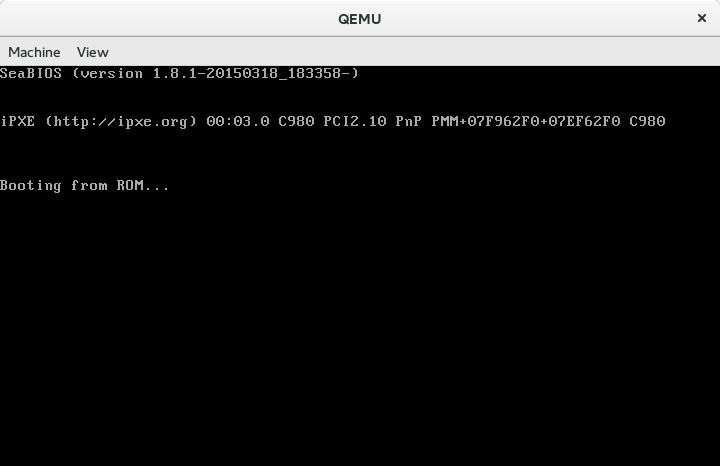
\includegraphics[scale=0.5]{../res/qemu-first-run.png}
\caption{qemu-system-i386 - Console \textit{QEMU}}
\end{figure}

Vous l'aurez remarqué, il ne se passe rien. La figure~\ref{fig:qemu_first_run} montre la console graphique ouverte par \textit{QEMU}. Nous allons rendre le noyau verbeux et afficher ses traces sur la console de \textit{QEMU} afin de comprendre ce qu'il se passe.

\subsection{Noyau verbeux}

\begin{figure}
\label{fig:menuconfig_enable_printk}
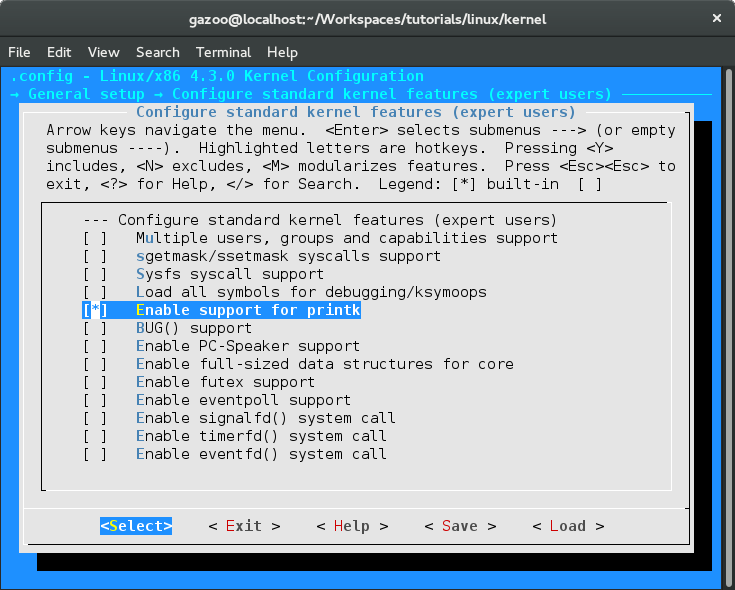
\includegraphics[scale=0.5]{../res/menuconfig-enable-printk.png}
\caption{menuconfig - Support de \textit{printk}}
\end{figure}

Pour rendre le noyau plus verbeux, activons les traces \textit{printk}. Sous le menu \textbf{General Setup}, puis \textbf{Configure standard kernel features (expert users)}, cochons la case \textbf{Enable support for printk} comme illustré par la figure~\ref{fig:menuconfig_enable_printk}.\\

\begin{figure}
\label{fig:menuconfig_enable_tty}
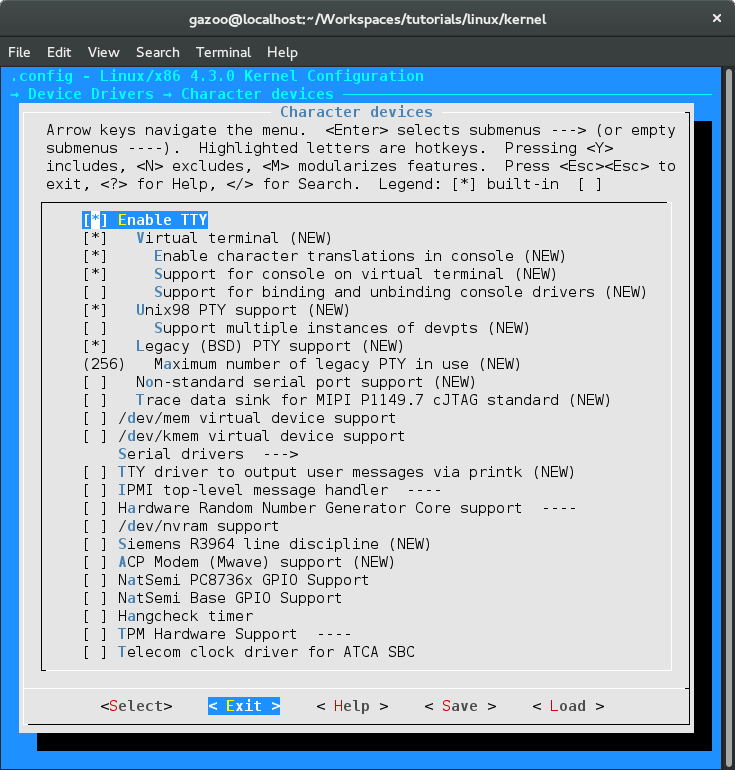
\includegraphics[scale=0.5]{../res/menuconfig-enable-tty.png}
\caption{menuconfig - Support de \textit{TTY}}
\end{figure}

\begin{figure}
\label{fig:menuconfig_enable_console}
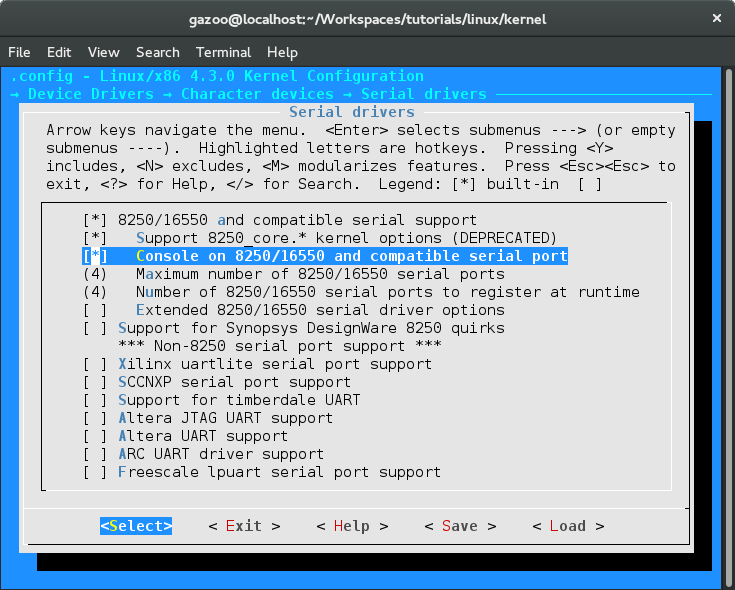
\includegraphics[scale=0.5]{../res/menuconfig-enable-console-on-8250-16550-serial-port.png}
\caption{menuconfig - Support de la console sur port série \textit{8250/16550}}
\end{figure}

Ensuite, configurons le projet pour compiler les pilotes utilisés par la console de \textit{QEMU}. Sur un \textit{PC}, \textit{QEMU} émule un port série compatible \textit{8250/16550}. Sous le menu \textbf{Device Drivers} puis \textbf{Character devices  --->}, cochons la case \textbf{Enable TTY}. Et, sous le nouveau sous-menu \textbf{Serial drivers  --->} cochons également la case \textbf{8250/16550 and compatible serial support} puis \textbf{Console on 8250/16550 and compatible serial port}. Referez vous aux figures~\ref{fig:menuconfig_enable_console} et \ref{fig:menuconfig_enable_tty}.\\

Deux nouveaux périphériques sont utilisables par le noyau :
\begin{itemize}
\item \textbf{console} et
\item \textbf{ttySx} ou \textit{x} représente un entier définissant le numéro du port série.
\end{itemize}

\subsection{QEMU}

Sur la ligne de commande de \textit{QEMU}, nous devons spécifier deux nouveaux paramètres :
\begin{itemize}
\item le premier pour émuler un port série (\textit{char-device}) et
\item le second pour surcharger la ligne de commande du noyau afin de lui spécifier le port série émulé comme étant la console du noyau.
\end{itemize}

\subsubsection{Émulation d'un port série}

L'émulation du port série se traduit par une série de deux paramètres :
\begin{itemize}
\item la création du périphérique de type \textit{isa-serial} : \lstset{language=sh}\lstinline{-device isa-serial,chardev=tty}
\item l'association \lstset{language=sh}\lstinline{-chardev stdio,id=tty}
\end{itemize}

\subsubsection{Surcharge de la ligne de commande du noyau}

Nous allons surcharger la ligne de commande du noyau en ajoutant une console via le paramètre \href{https://www.kernel.org/doc/Documentation/serial-console.txt}{\textbf{console=device,options}}.

\lstset{language=sh}\lstinline{-append console=ttyS0}

Et voilà !

\begin{verbatim}
$ qemu-system-i386 -kernel output/linux-x86/arch/x86/boot/bzImage -append "console=ttyS0" -serial stdio
Linux version 4.3.0 (gazoo@localhost.localdomain) (gcc version 5.1.1 20150618 (Red Hat 5.1.1-4) (GCC) ) #4 Mon Dec 7 17:18:49 CET 2015
x86/fpu: Legacy x87 FPU detected.
x86/fpu: Using 'lazy' FPU context switches.
e820: BIOS-provided physical RAM map:
BIOS-e820: [mem 0x0000000000000000-0x000000000009fbff] usable
BIOS-e820: [mem 0x000000000009fc00-0x000000000009ffff] reserved
BIOS-e820: [mem 0x00000000000f0000-0x00000000000fffff] reserved
BIOS-e820: [mem 0x0000000000100000-0x0000000007fdffff] usable
BIOS-e820: [mem 0x0000000007fe0000-0x0000000007ffffff] reserved
BIOS-e820: [mem 0x00000000fffc0000-0x00000000ffffffff] reserved
Notice: NX (Execute Disable) protection missing in CPU!
e820: last_pfn = 0x7fe0 max_arch_pfn = 0x100000
init_memory_mapping: [mem 0x00000000-0x000fffff]
init_memory_mapping: [mem 0x07800000-0x07bfffff]
init_memory_mapping: [mem 0x00100000-0x077fffff]
init_memory_mapping: [mem 0x07c00000-0x07fdffff]
127MB LOWMEM available.
  mapped low ram: 0 - 07fe0000
  low ram: 0 - 07fe0000
Zone ranges:
  Normal   [mem 0x0000000000001000-0x0000000007fdffff]
Movable zone start for each node
Early memory node ranges
  node   0: [mem 0x0000000000001000-0x000000000009efff]
  node   0: [mem 0x0000000000100000-0x0000000007fdffff]
Initmem setup node 0 [mem 0x0000000000001000-0x0000000007fdffff]
e820: [mem 0x08000000-0xfffbffff] available for PCI devices
clocksource: refined-jiffies: mask: 0xffffffff max_cycles: 0xffffffff, max_idle_ns: 7645519600211568 ns
Built 1 zonelists in Zone order, mobility grouping on.  Total pages: 32382
Kernel command line: console=ttyS0
PID hash table entries: 512 (order: -1, 2048 bytes)
Dentry cache hash table entries: 16384 (order: 4, 65536 bytes)
Inode-cache hash table entries: 8192 (order: 3, 32768 bytes)
Initializing CPU#0
Memory: 128016K/130552K available (730K kernel code, 96K rwdata, 112K rodata, 108K init, 196K bss, 2536K reserved, 0K cma-reserved)
virtual kernel memory layout:
    fixmap  : 0xfffe5000 - 0xfffff000   ( 104 kB)
    vmalloc : 0xc87e0000 - 0xfffe3000   ( 888 MB)
    lowmem  : 0xc0000000 - 0xc7fe0000   ( 127 MB)
      .init : 0xc10ee000 - 0xc1109000   ( 108 kB)
      .data : 0xc10b6cc9 - 0xc10ec0c0   ( 212 kB)
      .text : 0xc1000000 - 0xc10b6cc9   ( 731 kB)
Checking if this processor honours the WP bit even in supervisor mode...Ok.
NR_IRQS:16 nr_irqs:16 16
Console: colour VGA+ 80x25
console [ttyS0] enabled
tsc: Unable to calibrate against PIT
tsc: No reference (HPET/PMTIMER) available
tsc: Marking TSC unstable due to could not calculate TSC khz
Calibrating delay loop... 306.94 BogoMIPS (lpj=613888)
pid_max: default: 4096 minimum: 301
Mount-cache hash table entries: 1024 (order: 0, 4096 bytes)
Mountpoint-cache hash table entries: 1024 (order: 0, 4096 bytes)
Last level iTLB entries: 4KB 0, 2MB 0, 4MB 0
Last level dTLB entries: 4KB 0, 2MB 0, 4MB 0, 1GB 0
CPU: Intel QEMU Virtual CPU version 2.3.1 (family: 0x6, model: 0x6, stepping: 0x3)
Performance Events: Broken PMU hardware detected, using software events only.
Failed to access perfctr msr (MSR c2 is 0)
clocksource: jiffies: mask: 0xffffffff max_cycles: 0xffffffff, max_idle_ns: 7645041785100000 ns
clocksource: pit: mask: 0xffffffff max_cycles: 0xffffffff, max_idle_ns: 1601818034827 ns
clocksource: Switched to clocksource pit
platform rtc_cmos: registered platform RTC device (no PNP device found)
Serial: 8250/16550 driver, 4 ports, IRQ sharing disabled
serial8250: ttyS0 at I/O 0x3f8 (irq = 4, base_baud = 115200) is a 16550A
serio: i8042 KBD port at 0x60,0x64 irq 1
serio: i8042 AUX port at 0x60,0x64 irq 12
mousedev: PS/2 mouse device common for all mice
input: AT Translated Set 2 keyboard as /devices/platform/i8042/serio0/input/input0
input: ImExPS/2 Generic Explorer Mouse as /devices/platform/i8042/serio1/input/input3
Freeing unused kernel memory: 108K (c10ee000 - c1109000)
Kernel panic - not syncing: No working init found.  Try passing init= option to kernel. See Linux Documentation/init.txt for guidance.
Kernel Offset: disabled
---[ end Kernel panic - not syncing: No working init found.  Try passing init= option to kernel. See Linux Documentation/init.txt for guidance.
\end{verbatim}

Un noyau, c'est bien... mais le noyau ne constitue en rien un système complet ! Il manque la partie applicative appelé \textit{user-space}.

\clearpage
\listoffigures

\end{document}
